\chapter{Design}
This chapter summarizes the overall design of our approach to generating textual medical reports for X-ray images. The problem consists of multiple independent parts we need to deal with. For each of them, we we will present the fundamentals of our solution, along with description of related problematics and decisions made.

\section{Our approach}
As we already mentioned in the Chapter \ref{sec:RelatedWork}, the overall solution for the final medical report generation model is based on the \citet{alfarghaly2021automated}. We have chosen this approach for multiple reasons. The main reasons to use this work as the backbone for our thesis are following:
\begin{enumerate}
	\item In the work the state-of-the-art GPT-2 model is utilized as the language model. This gave us a great opportunity as there was none Czech GPT-2 model available at time this thesis began.
	\item The encoder is already fine-tuned to extract visual features for specific dataset.
	\item All solution source code is freely accessible on the github\footnote[1]{\url{https://github.com/omar-mohamed/GPT2-Chest-X-Ray-Report-Generation}}.
\end{enumerate}

As in most works for image captioning, the architecture is encoder-decoder based with an attention mechanism. The high-level solution architecture is depicted in Figure \hyperref[fig01:OmarArchitecutre]{2.1}.

\begin{figure}[h]\centering
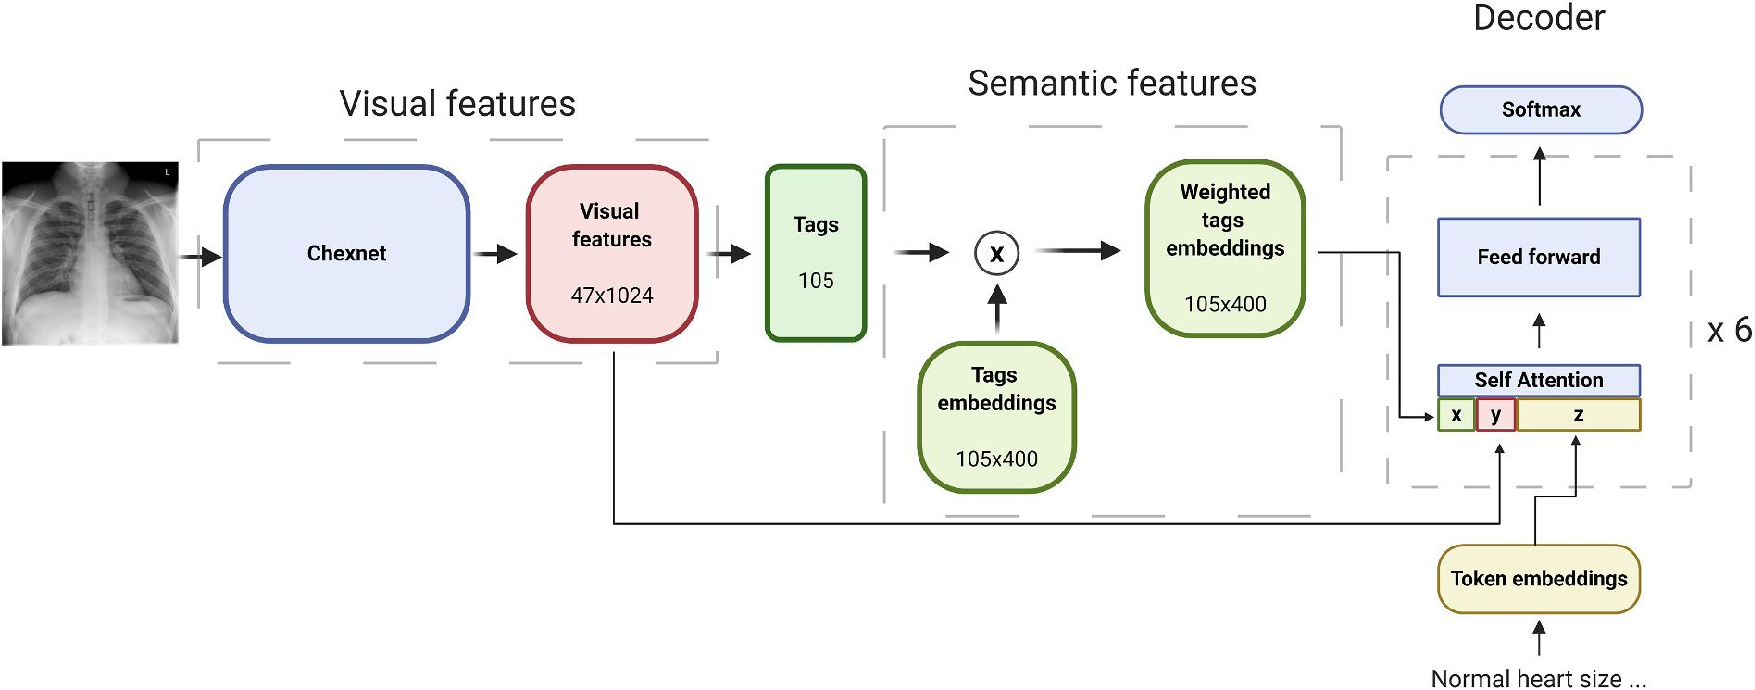
\includegraphics[width=145mm, height=57mm]{../img/OmarArchitecture}
\caption{Overall architecture used in our solution proposed in \citet{alfarghaly2021automated}.}
\label{fig01:OmarArchitecutre}
\end{figure}

\section{Czech GPT-2}
The aim of this work is to generate medical reports in the Czech language. In the previous parts, we decided to use the GPT-2 as the language model. However at the time of the beginning of this work, no Czech GPT-2 model was freely available and thus it was essentially necessary to create one. This section describes all the steps needed for fine-tuning the small English GPT-2 to the Czech language. Respectively, we train two versions of the Czech GPT-2 model. One trained on the general Czech textual data and one specialized specifically on Czech medical texts.

\subsection{Data}
In this section we will describe the possible data applicable for training of both the general and medical Czech GPT-2 model together with the decision made about the final data selection and data cleaning.

\subsubsection{General}
For the training of general Czech GPT-2 we have a plenty of data options we can choose from. However, there are important properties of the data we need to sastisfy. As we are transfer learning from English to Czech language we need to have sufficiently large data, so we ensure the GPT-2 will learn properly syntactical and semantical information. Moreover, the data have to be also heterogeneous enough, so the model can capture different types of information and not just for example newspaper articles from a specific area. In order to create a good enough general model we need to meet these criteria.\\

Several different datasets were investigated and tested for the training of the general Czech GPT-2 model.
\paragraph*{Czech Wikipedia} ~\\
\indent The first data we used for training the model is the Czech~Wikipedia~dump\footnote[2]{\url{https://dumps.wikimedia.org/cswiki/latest/cswiki-latest-pages-articles.xml.bz2}}. After extraction, the total size of the dataset is approximately 800 MB of raw text. The advantages of this dataset are its easy accessibility and fairly clean data quality. On the other hand, the data are very homogeneous despite the various topics. Each article is written in the general descriptive style. Moreover the data themself are not large enough, the trained model made many both syntactical and semantical mistakes during the text generation.

\paragraph*{Balanced Czech National Corpus} ~\\
\indent Another possibility was to use a balanced version of the Czech National Corpus\citep{11234/1-4635} as the original is composed mainly of journalistic articles. The balanced version tries to equalize the amount of data from each category. These categories include \textit{journalism}, \textit{poetry}, \textit{prose}, \textit{educational literature} etc. The major advantage of this dataset is its purity, the texts are syntacticaly correct without any undesirable non-Czech elements and written in the standard Czech language. The dataset does not have any significant downsides and the trained model understood Czech language without any significant ailments. In total, the dataset is comprised of 3,3 GB of raw text.

\paragraph*{OSCAR} ~\\
\indent OSCAR, from the \citet{ortiz-suarez-etal-2020-monolingual}, is a huge deduplicated multilingual corpus created from the Common~Crawl~corpus\footnote[3]{\url{https://commoncrawl.org/}} providing data for 166 different languages and available directly in the huggingface datasets library\footnote[4]{\url{https://huggingface.co/datasets/oscar}}. It consists of the text scraped from websites of very different kinds and thus the data are heteregeneous enough. Moreover, its huge size, as the czech part of the dataset occupies a total of 24 GB of raw text, is another major benefit. On the other hand, because the data are automatically scraped, they carry a noise in them. Besides that, not negligible part of the text are in the non-standard Czech language as the data come from diverse web sources such as forums etc. Nevertheless, the disadvantages are outweighed by the huge size of the corpus and together with following filtering of the text:
\begin{enumerate}
	\item We take only text that are at least 1200 characters longs as these texts tend to be longer articles written in the standard Czech language instead of advertisements, incomple texts etc.
	\item Any text containing control character are filtered out, because the text contains generally undesirable content.
\end{enumerate}

\paragraph*{Conclusion} ~\\
\indent We analyzed various datasets along with their overall properties. Furthermore, the advantages and disadvantages of each were discussed. As a result, we have chosen the \textbf{OSCAR} dataset due to its size and heterogeneity. The \textbf{Wikipedia} is too small and homogeneous. On the other hand the \textbf{Balanced Czech National Corpus} is heterogeneous enough, however it is an almost order of magnitude smaller than \textbf{OSCAR}.

\subsubsection{Medical}
Since we have a trained general Czech GPT-2 model from the previous section that already understands a Czech language, the final fine-tuning for medical environment does not require that much data. We need to specialize the model to understand the mecial environment inherently. For this purpose, we use a subset of the UFAL~Medical~Corpus~v. 1.0\footnote[5]{\url{https://ufal.mff.cuni.cz/ufal\_medical\_corpus}}. These data are further filtered to remove any inappropriate characters, lines and redundant structures. As a result, the data contain a total of 100 MB of raw medical texts. The texts comprise of general medical descriptions, articles and package leaflets for medicines.

\subsection{Training}
TODO - Popsat postup tréninku podle příspěvku(popis - obecně, trénování tokenizeru, postupné trénování) + learning rate finder(popis, obrázek) + diff lear. rates(popis - 4 skupiny) + ta trénovací křivka(popis - rozdíl oproti klasickýmu, obrázek), popsat ještě rozdíl mezi originállním přístupem a novým(gradual vs full)

\section{Medical dataset translation}
For machine learning in general and NLP tasks especially, the data quality is the alpha and omega of the performance of the final model. Since, as we have already mentioned in the Chapter \ref{sec:CzechData}, we do not have any Czech data directly for the medical examinations of X-rays, to obtain Czech data we must arrange ourselves in a different way. One potential way is to create a new artificial dataset using machine translation of existing datasets. This section discusses the required steps to build a quality dataset using translation.

\subsection{Translator choice}
In the previous part of the text, specifically in the Chapter \ref{sec:Translators}, we already discussed all possibilities for automatic translation. Our final choice for the translator is the CUBBITT as it provides REST API unlimited in the number of requests and volume.

\subsection{Preprocessing}
\label{sec:DataPreprocessing}
The most important part of our machine translation process is the preprocessing of the input text. We already outlined in the Chapter \ref{sec:datasets} that the data contain some noise in them as we are dealing with reports in natural language. Moreover, we will use CUBBITT translator, that doest not perfom auto-correction itself and cannot translate some patterns at all as we described in the Chapter \ref{sec:Cubbitt}. For these purposes we incorporate preprocessing before the translation as it would be beneficial to have all texts in standardized form in order to firstly, help CUBBITT with translation to get the report correctly translated, and secondly to ensure that our model receives and process all the data in a indentical report format.\\

Our preprocessing pipeline encompasses of following procedures. Some of them are dealing with general CUBBITT issues and other with specifics of the medical data.

\subsubsection*{Line starts}
First of all we start with a very simple procedure. We analyze all lines of the report and delete all white characters common for all lines on both ends. The purpose of this modification is to standardize the report format, while preserving its structure.

\subsubsection*{Anonymous sequences}
Inasmuch as the whole datasets are anonymized due to the legal reasons and privacy protection, the reports contain \qq{anonymous sequences}, such as \qq{XXXX} or \qq{\underline{{ }{ }{ }{ }{ }}}, denoting places with original private information about patients. However, these sequences can be attached to surrounding words forming undesirable words. As we already said, the CUBBITT does not auto-correct its input automatically, so these inputs will not be handled in any special way and therefore not translated. For this reason, we separate these sequences to form independent words.

\subsubsection*{Units}
Subsequent form of correction that we perform is the separation of numbers and units attached to them. In addition, this also includes general cases, where the number and subsequent word are glued together, while keeping specific medical terms with a similar structure. This is associated with the following step, as the units will not be true-cased properly without this procedure.

\subsubsection*{True-casing}
The most imporant part of the whole preprocessing pipeline is true-casing of the input text. This adjustment is necessary for two essential reasons. CUBBITT has problems with translation of any uppercase texts in general. Capturing the true-case of a text is a complex problem requiring either a large statistical language dictionary or a trained model in order to properly determine the case.\\

As medical reports are very specific area, the existing solutions for general text true-casing is inapplicable. Medical reports contain a lot of abbreviations and acronyms, which can be often confused with ordinary english words. Training the model for medical true-casing requires even more specific data for a certain domain, because in different contexts the common words can be treated differently. Moreover, obtaining flawless data to cover the entire specific domain is a challenging task. For these reasons, we chose the way of a statistical dictionary. Before the translation of the dataset begins, we create a statistical dictionary from the whole dataset containing the most often used form of every word. We also count with some exceptions, such as headings, that in some datasets can be in uppercase only.\\

Using the created dictionary, we deal with all uppercase words to assign them the proper form. The results of the true-casing preprocessing are demonstrated in the following examples:
\begin{itemize}
	\item (1a) \qq{EXAMINATION: CHEST (PORTABLE AP)} $\rightarrow$ \\ \phantom{(1a)} \qq{PŘEZKOUŠENÍ: CHEST (PORTABLE AP)}
	\item (1b) \qq{Examination: Chest (portable AP)} $\rightarrow$ \\ \phantom{(1b)} \qq{Vyšetření: Hrudník (přenosný~AP)}
	\item (2a) \qq{SMALL RIGHT PLEURAL ABNORMALITY} $\rightarrow$ \\ \phantom{(2a)} \qq{MALÉ PRÁVO PLEURÁLNÍ ABNORMALITY}
	\item (2b) \qq{Small right pleural abnormality} $\rightarrow$ \\ \phantom{(2b)} \qq{Malá pravá pleurální abnormalita}
\end{itemize}

\subsubsection*{Paragraphs structure}
In some of the medical reports the section headings and corresponding texts do not begin on the same lines. We adjust these situations to a form where each heading and the text belonging to it always starts on the same line, for two reasons. Firstly, we want to normalize the report structure in general and secondly, we want to move the section content as close as possible to the heading, so the translator and even the final model have the context close to each other.

\subsubsection*{Capitalization}
Another part of the preprocessing pipeline is a simple capitalization of each heading and each sentence in the report. This text capitalization process helps CUBBITT not only in the case of medical data, but in general during the translation process of some texts to better understand the boundaries between sentences.

\subsubsection*{Time}
One of the patterns that CUBBITT doest not recognize nor auto-corrects itself in general are times. This applies both, to the specification of hours and minutes, and to the  part of the day specification. If any of these parts are incorrectly formatted, the time will we translated incorrectly or not translated at all, and thus we would lose some information or it could damage the fluency of the translated text. For these reasons, we apply preprocessing to normalize all times. We can see the difference in the following examples:
\begin{itemize}
	\item \qq{Chest radiograph at 1045PM} $\rightarrow$ \qq{Rentgen hrudníku v 1045PM}
	\item \qq{Chest radiograph at 10:45 PM} $\rightarrow$ \qq{Rentgen hrudníku ve 22:45}
\end{itemize}

\subsubsection*{White spaces}
After all previous procedures, we apply one last very simple final modification, namely, we squash all the whitespace characters inside each line into a single space, while maintaining the format from the very first preprocessing step described above. This step is performed only for normalization purposes.

\subsubsection*{Lowercasing}
The last preprocessing procedure we will mention is lowercasing of the whole text followed by capitalizing the first word of each sentence. This is a separate procedure that was used in the earlier phases of elaboration of this work as CUBBITT has problem with uppercased word as we already mentioned.















